\chapter{Biolomorfismi}
Abbiamo distinto le superfici di Riemann in tre tipi:
\begin{itemize}
\item La superficie sferica $\hat\bbC$;
\item Le superfici euclidee, ottenute quozientando $\bbC$;
\item Le superfici iperboliche, ottenute da quozienti del disco $D$.
\end{itemize}

Esistono delle condizioni molto stringenti sulle mappe tra superfici di Riemann di tipo diverso, date dal sollevamento delle mappe ai rivestimenti universali.

\begin{proposizione}
Ogni mappa olomorfa da una superficie sferica a una euclidea è costante. Allo stesso modo, ogni mappa biolomorfa da una superficie euclidea a una iperbolica è costante.
\end{proposizione}

\begin{proof}
Siano $S_1$, $S_2$ e $S_3$ tre superfici, rispettivamente sferica, euclidea e iperbolica, e siano $f: S_1 \rar S_2$, $g: S_2 \rar S_3$ mappe biolomorfe, come nel diagramma.

\[
    \begin{diagram}
        \hat \bbC 		& \rTo^{\tilde f} 	& \bbC 			& \rTo^{\tilde g} 	& D 	\\
        \dTo>{\pi_1}	&					& \dTo>{\pi_2}	&					& \dTo>{\pi_3}	\\
        S_1				& \rTo^f 			& S_2 			& \rTo^g 			& S_3
    \end{diagram}
\]

Poichè sia $\hat\bbC$ sia $\bbC$ sono semplicemente connessi, per il solito lemma $f \circ \pi_1$ e $g \circ \pi_2$ si sollevano a $\tilde f, \tilde g$.

Ma $\tilde f$, ristretta a $\bbC$, è una mappa intera (olomorfa su $\bbC$) limitata (perchè all'infinito deve tendere ad $f(\infty)$). Quindi per Liouville è costante.
Stesso discorso vale per $\tilde g$, che è olomorfa su $\bbC$ ed è limitata (ha immagine contenuta nel disco). Quindi anche $f$ e $g$ devono essere costanti.
\end{proof}

\notamargine{Inoltre, potete mostrare che non vi sono mappe olomorfe da superfici sferiche a superfici iperboliche, utilizzando le carte su $\hat\bbC$ ed il teorema di Liouville su queste. Nell'altro verso invece ve ne sono di non costanti, in particolare potete prendere l'immersione da $D$ in $\bbC$ e quella da $\bbC$ in $\hat\bbC$}


Consideriamo ora una mappa olomorfa $f:X\to Y$ tra superfici di Riemann, e siano $\tilde X,\tilde Y$ i due rivestimenti universali; diciamo che $X=\tilde X / G_X,Y=\tilde Y / G_Y$ con le rispettive proiezioni $\pi_X,\pi_Y$.\\
Costruiamo il seguente diagramma
\[
    \begin{diagram}
        \tilde X  		& \rTo^{\tilde f} 	& \tilde Y 		 	\\
        \dTo>{\pi_X}	&					& \dTo>{\pi_Y}		\\
        X   			& \rTo^f 			& Y
    \end{diagram}
\]
dove $\tilde f$ è il sollevamento della mappa olomorfa $f\circ\pi_X:\tilde X\to Y$.\\
Vediamo che anche $\tilde f$ deve essere olomorfa.\\
Sia $g\in G_X$, allora deve essere $\tilde f(gz)=\gamma(z)\tilde f(z)$ con $\gamma(z)\in G_Y$ in modo da far commutare il diagramma. Vediamo che in realtà $\gamma$ è indipendente da $z$, poiché $G_Y$ è discreto.\\
\begin{osservazione}
    Se viceversa vale la condizione $\forall g\in G_X\exists\gamma\in G_Y: \tilde f(gz)=\gamma\tilde f(z)$, allora la mappa $f$ è olomorfa.
\end{osservazione}

Infine, se $f$ era un biolomorfismo, ovvero possiede un'inversa $g$ olomorfa, possiamo sollevarla a $\tilde g$ che soddisfa la stessa condizione.\\
\newthought{Attenzione!} La $\tilde g$ non è l'inversa di $\tilde f$, ma in generale varrà solamente $\tilde f\circ\tilde g\in\Aut(\tilde Y)$ e $\tilde g\circ\tilde f\in\Aut(\tilde X)$




\section{Biolomorfismi di tori}
Restringiamoci ora ai tori, ovvero quozienti $\quotient{\bbC}{L}$ con $L$ reticolo di rango $2$. Dimostreremo che una mappa tra due tori $T_1 = \bbC/L_1$ e $T_2 = \bbC/L_2$ deve essere della forma $f(z)=\alpha z + \beta$.\notamargine{D'ora in poi faremo spesso confusione tra un numero complesso e la sua classe di equivalenza.}

\notamargine{Attenzione, molti matematici usano nella definizione di reticolo il fatto che il reticolo abbia la stessa dimensione dello spazio vettoriale in cui è contenuto, nel nostro caso è contenuto in $\bbC$ che ha dimensione reale $2$.}

\begin{osservazione}
Se prendiamo reticoli omotetici, ovvero due reticoli $L$ e $\lambda L$, con $\lambda \in \bbC\minus\{ 0\}$, si ha che i tori ottenuti sono biolomorfi. (La mappa moltiplicazione per $\lambda \quad \bbC \rightarrow \quotient{\bbC}{\lambda L} \hquad z\ \mapsto [\lambda z]_{\lambda L} $ è ben definita e passa al quoziente $\quotient{\bbC}{L}\rightarrow \quotient{\bbC}{\lambda L}$, che è olomorfa e ha come inversa olomorfa la moltiplicazione per $\lambda^{(-1)}$).
\end{osservazione}

\begin{proposizione}Sia $f:T_1\rightarrow T_2$ olomorfa non nulla tra tori, con $T_i=\quotient{\bbC}{L_i},\hquad i\in \{ 1,2\}$, allora $\exists\alpha\neq0 \hquad \alpha L_1\subseteq L_2$.
\end{proposizione}
\begin{proof} Siano $\pi_i,\hquad i\in \{ 1,2\}$ le mappe di proiezione.
    \[
        \begin{diagram}
            \bbC            & \rTo^{\tilde f} 	& \bbC 		 	\\
            \dTo>{\pi_1}	&					& \dTo>{\pi_2}		\\
            T_1   			& \rTo^f 			& T_2
        \end{diagram}
    \]
Si ha che la mappa $f\circ\pi_1: \bbC\rightarrow T_2$, siccome $\bbC$ è semplicemente connesso, si solleva a $\tilde{f}$ olomorfa (non necessariamente unica).
Prendendo $x_1\in T_1$, $z$ t.c. $\pi_1(z)=x$, allora $\pi_2\circ\tilde{f} (z) = f\circ \pi_1 (z)= f(x)$, quindi $\pi_2\circ \tilde{f}$ non dipende dal rappresentante $z$, ovvero $\pi_2\circ \tilde{f} (z+\lambda_1)=\pi_2\circ \tilde{f} (z)\hquad \forall \lambda_1\in L_1$.
Ma allora $\tilde{f} (z+\lambda_1) - \tilde{f} (z) \in L_2 \hquad \forall \lambda_1 \in L_1$.
Ma essendo $L_2$ discreto e $\tilde{f}$ continua si ha che $\tilde{f}(z+\lambda_1)=\tilde{f}(z)+c(\lambda_1)\hquad \forall z\in\bbC$, con $c(\lambda_1)\in L_2$ costante dipendente solo da $\lambda_1$.
Derivando l'ultima uguaglianza, si ha che $\tilde{f}'(z+\lambda_1)=\tilde{f}'(z) \hquad\forall \lambda_1\in L_1$.
Perciò la funzione $\tilde{f}'$ si quozienta ad una funzione  $T_1\rightarrow \bbC$ ne segue che la sua immagine è un compatto, quindi limitato e quindi per Liouville è costante.
Perciò $\tilde{f}$ è lineare, $\tilde{f}(z)=\alpha z+\beta$.
Sostituendo questo in $\tilde{f} (z+\lambda_1) - \tilde{f} (z) \in L_2 \hquad \forall \lambda_1 \in T_1$ si trova $\alpha L_1\subseteq L_2$.
\end{proof}

\notamargine{Vedi anche Elliptic Function, Lang, pagina 14}

\begin{osservazione}
Non è detto che la mappa $f$ sia biunivoca come mappa $T_1\rightarrow T_2$, anche se la mappa "sopra" $\tilde{f}$ lo è.
\end{osservazione}

Viceversa se si ha $\alpha$ che soddisfa $\alpha L_1 \subseteq L_2$  allora la mappa moltiplicazione per $\alpha: \quad \bbC \rightarrow \quotient{\bbC}{L_2} \hquad z\ \mapsto [\alpha z]_{L_2} $ è ben definita e passa al quoziente $\quotient{\bbC}{L_1}\rightarrow \quotient{\bbC}{L_2}$.

\begin{osservazione}
\begin{itemize}
\item Tolta la traslazione $\beta$ (è un automorfismo di $\bbC$) le mappe indotte sui tori sono omomorfismi di gruppi.
\item A livello algebrico i tori hanno una realizzazione come gruppi con legge di gruppo razionale.
La mappa che manda tori in curve algebriche sono funzioni trascendenti (esempio esponenziale). MAH
\end{itemize}
\end{osservazione}


\begin{fatto} Considero $f$ omomorfismo di gruppi e biolomorfismo, quindi indotta da $\tilde{f}=\alpha z$. Allora $\alpha L_1=L_2$.
\end{fatto}
\begin{proof}
Sia $[z]_{L_1} \mapsto [\alpha z]_{L_2}$ indotta dalla moltiplicazione per $\alpha$, se è invertibile considero gli elementi $[\frac{\lambda_2}{\alpha}]_{L_1}, \lambda_2 \in L_2$, allora questi vengono mandati in $0$ dalla mappa $f$, poiché è iniettiva, ovvero tutti i $\frac{\lambda_2}{\alpha}$ devono stare in $L_1$, ovvero $\frac{1}{\alpha} L_2 \subseteq L_1 \Rightarrow L_2 \subseteq \alpha L_1$.
Quindi siccome sapevo già che $\alpha L_1 \subseteq L_2$ ho trovato che $\alpha L_1 =L_2$.
\end{proof}

\begin{esercizio} Sia $f$ omomorfismo olomorfo tra tori, allora il nucleo è un insieme finito, ed è misurato da $\quotient{L_2}{\alpha L_1}$ (quoziente di due gruppi, uno sottogruppo di quell'altro).
\end{esercizio}

\begin{esercizio}
L'indice di un reticolo di rango $2$ contenuto in un altro è finito.
\end{esercizio}

\notamargine{Suggerimento: prendere gli elementi di base.\\ Esempio: $n\bbZ \oplus m\bbZ \le \bbZ \oplus \bbZ$ ha indice $nm$.}

\begin{osservazione}
\begin{itemize}
\item Si è dimostrato che due tori sono biolomorfi se e solo se i reticoli sono omotetici, in formule $T_1\cong T_2 \iff \exists \alpha\in\bbC^* \alpha L_1=L_2$.
\item Nota che due Tori sono sempre isomorfi come spazi topologici, come varietà reali e come gruppi di Lie (gruppi analitici reali).
\item Che siano omeomorfi come superfici di Riemann, ovvero che i reticoli soddisfino $\exists \alpha\in\bbC^* \alpha L_1=L_2$  è una condizione molto forte
\end{itemize}
\end{osservazione}


\section{Spazio dei parametri}
Si ha che la condizione sui reticoli ci permette di analizzare lo spazio di parametri per i tori.

Preso un reticolo generico $L=\omega_1 \bbZ + \omega_2 \bbZ$ con $\Im \frac{\omega_1}{\omega_2} \ne 0$ si ha che, se si sceglie l'orientazione con $\Im \frac{\omega_1}{\omega_2}>0$ (a meno di scambiare $\omega_1$ con $\omega_2$), il toro è omotetico a $\frac{1}{\omega_2} L= \tau \bbZ+ \bbZ$, con $\tau=\frac{\omega_1}{\omega_2} \in \mathcal{H}$.

La base in $\{\omega_1, \omega_2 \}$ non è determinata, infatti posso fare qualsiasi cambio di base con matrice $	\begin{pmatrix} a & b \\ c & d \end{pmatrix}$ con $a,b,c,d \in \bbZ$ e $ad-bc=\pm 1$. (invertibile)

Se però considero le basi orientate, ovvero se dalla base $\{\omega_1, \omega_2 \}$ con $\Im \frac{\omega_1}{\omega_2}>0$ passo alla base $\{\omega_1', \omega_2' \}$ con $\Im \frac{\omega_1'}{\omega_2'}>0$, allora si ha che $\tau'=\frac{\omega_1'}{\omega_2'}=\frac{a\tau +b}{c\tau+d}=\frac{ac |\tau |^2+bd+ad\tau +bc \bar\tau}{|c\tau+d|^2}$, quindi $\Im\tau'=\frac{(ad-bc)}{ |c\tau+d|^2} \Im(\tau-\bar\tau)$ ma siccome $\Im(\tau-\bar\tau)=\frac{(\tau-\bar\tau)-\overline{(\tau-\bar\tau)}}{2i}=\frac{2\tau-2\bar\tau}{2i}=2(\Im\tau)$ allora $\Im\tau'$ ha lo stesso segno del determinante.

Cioè abbiamo visto che le matrici di cambio di base, se conserviamo l'orientazione, sono le matrici di $SL_2(\bbZ)$, ne risulta che lo spazio dei tori complessi di dimensione complessa $1$ a meno di biolomorfismo è $\quotient{\mathcal{H}}{SL_2(\bbZ)}$.

\begin{osservazione}
\begin{itemize}
\item Non è ovvio vedere cosa sia quel quoziente.
\item Topologicamente è $\bbC$.
\item $SL_2(\bbZ)$ ha dei punti fissi, quindi il quoziente non è una superficie di Riemann con la mappa indotta da $\mathcal{H}$.
\item per avere superfici di Riemann devo prendere gruppi che soddisfano le famose proprietà, per esempio $\Gamma (2)$.
\item Le matrici di quel tipo sono numerabili, $\mathcal H$ ha la cardinalità del continuo, quindi il quoziente ha la cardinalità del continuo.
\item Un dominio fondamentale (contiene un punto per ogni classe di biolomorfismo di tori) è dato da $\{ x+iy | -\frac{1}{2}<x<\frac{1}{2}, y>\sqrt{1-x^2}\}$. Vedi \ref{fig:2}
\end{itemize}
\end{osservazione}
Una trattazione più approfondita di queste cose avverrà nell'ultima parte sulle funzioni modulari.


\begin{figure}[h]
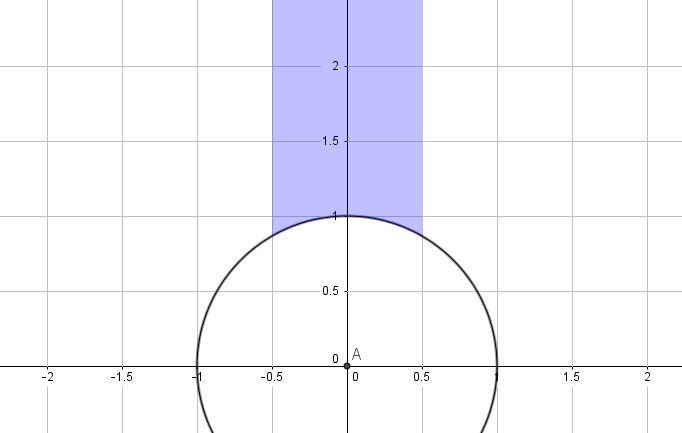
\includegraphics[width=8cm]{lezione-161024-fig3}
\caption{Dominio fondamentale}\label{fig:2}
\end{figure}

\chapter{Leggi di gruppo olomorfe}

\begin{definizione}
Una legge di gruppo olomorfa su una superficie di Riemann $S$ è una legge di gruppo in cui la moltiplicazione e l'inverso sono mappe olomorfe rispettivamente da $S \times S$ a $S$ e da $S$ a $S$ (per un'opportuna definizione di mappa olomorfa da una varietà bidimensionale).
\end{definizione}

Su un toro abbiamo un'ovvia legge di gruppo ereditata dalla somma su $\bbC$. Inoltre possiamo mettere una legge di gruppo isomorfa, in cui cambio l'origine. Questo si può fare in generale: data la moltiplicazione $\cdot$ su un gruppo $G$, posso definire l'operazione $g * h = g\cdot a^{-1}\cdot h$, con $a\in G$. Allora $(G,*)$ ha $a$ come origine, e ho l'ovvio isomorfismo tra $(G,\cdot)$ e $(G,*)$ dato da $g\mapsto g\cdot a$.

\section{Leggi di gruppo sul toro}

\begin{proposizione}
A meno di cambi di origine, ho una sola legge di gruppo olomorfa sul toro $T$.
\end{proposizione}

\begin{proof}
Sia $x \in T$, sia $*$ una legge di gruppo e sia senza perdita di generalità $0$ l'elemento neutro. Consideriamo la funzione $\phi_x: z \mapsto x * z - x$.

Questa è una mappa olomorfa tra tori, e sappiamo che deve essere della forma $z \mapsto \alpha z + \beta$. Ma $\phi_x(0)=0$, quindi $\beta=0$. Sia quindi $c_x \in \bbC$ tale che $\phi_x(z)=c_xz$.

Quindi abbiamo, riarrangiando i termini della definizione
\[
 x*z = \phi_x(z) + x = c_xz + x
\]
(ricordiamo che si tratta di numeri complessi modulo il reticolo $L$).

Fissiamo ora $z_0\ne 0$. $c_x$ è una funzione olomorfa in $x$, infatti, detta $f(\zeta) = \zeta * z_0$, vale
\[
    f(\zeta) = \zeta + c_\zeta z_0 + \lambda, \lambda \in L
\]
stavolta pensata su $\bbC$. Quindi posso ricavare $c_\zeta$, e dato che $f$ è olomorfa per ipotesi, ottengo quello che volevo.

D'altra parte, fissato un qualsiasi $\lambda \in L$, allora $c_x\lambda \in L \; \forall x$, quindi poichè $x \mapsto c_x \lambda$ è olomorfa a valori in un discreto, deve essere localmente costante e quindi costante. Sia quindi $c=c_x$.

Ponendo $x=0$ ottengo che $\phi_0(z) = cz = z$, da cui $(c-1)z$ sta nel reticolo per ogni $z$, e quindi $c=1$.

\end{proof}

\section{Leggi di gruppo su $D$}

\begin{teorema}
Il disco unitario $D$ in $\bbC$ non ammette una struttura di gruppo olomorfa
\end{teorema}

\begin{proof}
Per assurdo; ci sono due possibili vie.\\
Conoscendo i gruppi di Lie, basta considerare la mappa esponenziale dal tangente nel disco: dovrebbe essere una mappa non costante da $\bbC$ nel disco. \hfill \Lightning \\
Altrimenti, sia $\star : D\times D \rar D$ una legge di gruppo olomorfa. Sia inoltre $x^{*}$ l'inverso di $x$ per $\star$. Senza perdita di generalità, si può supporre che $0 \in D$ sia l'elemento neutro.
Allora $\forall x\in D$ la mappa $L_{x}: z\mapsto x\star z$ è un automorfismo olomorfo. \\
Dunque,  $$x\star z = c(x)\frac{z -a(x)}{1- \overline{a}(x) z}$$
con $|c(x)|\equiv 1$ e $a:D \rar D$.\\
Per $z=0$ si ha $x=-c(x)a(x)$.\\
Per $z=a(x)$ si ha $x*a(x)=0$ $\Rar$ $a(x)=x^{*}$ $\Rar$ $a(x)$ è olomorfa $\Rar$ (per $x\neq 0$) $c(x)=-\frac{x}{x^{*}}$ $\Rar$ $c(x)$ è olomorfa per $x\neq 0$, ma $|c(x)| \equiv 1$ $\Rar$ per il teorema della mappa aperta deve essere $ \ c(x) \equiv k \neq 0$. Da cui $a(x)= -\frac{x}{k}$.\\
Allora, $$x\star 1/2 = k\frac{1-2a(x)}{2-\overline{a}(x)}$$
ma questa non è olomorfa ( $\overline{a}(x)$ non lo è, il resto sì).

\end{proof}

\section{Classificazione delle leggi di gruppo olomorfe}
Vogliamo ora classificare tutte le leggi di gruppo sulle superfici di Riemann. Per farlo useremo ancora una volta i rivestimenti, nel modo seguente:

\begin{lemma}
Sia $X$ un gruppo topologico con $\mu : X\times X \rar X$ legge di gruppo. Sia inoltre $p :\widetilde{X} \rar X$ il rivestimento universale.
Allora $\mu$ si solleva ad una $\tilde{\mu} : \widetilde{X} \times \widetilde{X} \rar \widetilde{X}$ che rende $\widetilde{X}$ un gruppo topologico.
\end{lemma}

\begin{proof}

            \begin{diagram}
                \widetilde{X}\times\widetilde{X}	& \rTo^{\widetilde{\mu}} 	& \widetilde{X}	\\
                \dTo<{p \times p}	&					& \dTo>{p}\\
                X\times X				& \rTo^\mu 		& X
            \end{diagram}

\noindent Sia $e \in X$ l'identità di $X$ e sia $\tilde{e} \in \widetilde{X}$ un punto t.c. $p(\tilde{e})=e$. Prodotto di semplicemente connessi è semplicemente connesso, dunque la mappa $\mu \circ (p \times p)$ solleva ad una mappa $\widetilde{\mu}$ che chiude il diagramma. Basta ora mostrare che $\widetilde{\mu}$ è una legge di moltiplicazione {\it (un po' di verifiche emozionantissime)}.\\

{\bf Elemento neutro:}
    \begin{diagram}
        \{\tilde{e}\}\times\widetilde{X}	& \rTo^{\widetilde{\mu}}_{\pi_{2}} 	& \widetilde{X}	\\
        \dTo<{p \times p}			&					& \dTo>{p}\\
        \{e\}\times X				& \rTo^\mu 				& X
    \end{diagram}

\noindent Per restrizione, $\tilde{\mu}$ chiude il diagramma. Ma anche la proiezione sul secondo fattore fa commutare il quadrato; per unicità del sollevamento a punto base fissato si ha che $\tilde{\mu}(\tilde{e}, \bullet) \equiv \pi_{2}(\bullet)$. Analogamente si ha che $\tilde{\mu}(\bullet, \tilde{e}) \equiv \pi_{1}(\bullet)$ e dunque $\tilde{e}$ è elemento neutro per $\tilde{\mu}$.

{\bf Associatività} e {\bf inverso} si ottengono in maniera del tutto analoga (cioè sfruttando l'unicità del sollevamento).
\notamargine{Per l'associatività utilizzare la diagonale sulla faccia del cubo}
\end{proof}

Abbiamo inoltre mostrato che i tori ammettono come unica struttura di gruppo olomorfo quella di gruppo quoziente di $\bbC$ sul reticolo $L$.

\begin{osservazione}
Sia $G$ un gruppo olomorfo. $\forall g \in G$ le traslazioni $L_{g}:z\mapsto g\star z$ e $R_{g}:z\mapsto z\star g$ sono mappe biolomorfe; se $g\neq e$, allora non hanno punti fissi.\\
Infatti per la struttura di gruppo, l'inversa di $L_g$ è semplicemente $L_{g^-1}$, che è ancora olomorfa.\\
Inoltre se fosse $g\star z = z$ per qualche $g,z$ dato che siamo in un gruppo possiamo invertire $z$ e ottenere $g=e$.
\end{osservazione}

\begin{proposizione}
La sfera di Riemann $\bbP_{1}\bbC $ non ammette strutture di gruppo olomorfo.
\end{proposizione}
\begin{proof}
    Supponiamo per assurdo che $\exists \star: \bbP^1\bbC \times \bbP^1\bbC \rar \bbP^1\bbC$ legge di gruppo (ed olomorfa).\\
    Allora le traslazioni $L_x$ definite da $z \mapsto x \star z \in \Aut(\bbP^1\bbC)$ sono automorfismi di $\hat\bbC$ per la struttura complessa, ovvero della forma $z\mapsto\dfrac{az+b}{cz+d}$ con $ad-bc\neq0$, e quindi come abbiamo visto hanno sempre almeno un punto fisso.
    Questo è assurdo per l'osservazione precedente, in quanto $\hat\bbC$ ha almeno due punti.
\end{proof}

\begin{proposizione}
L'unica struttura di gruppo olomorfo su $\bbC$ è quella data dall'addizione.
\end{proposizione}
\begin{proof}
    Supponiamo per assurdo che $\exists \star: \bbC \times \bbC \rar \bbC$ legge di gruppo olomorfa. Diciamo che l'elemento neutro sia lo $0$.\\
    Fissiamo $z_0\in\bbC$; allora la traslazione $L_{z_0}$ definita da $z \mapsto z_0 \star z \in \Aut(\bbC)$ è un automorfismo di $\bbC$ per la struttura complessa, ovvero della forma $z\mapsto az+b$ con $a\neq0$.
    Inoltre grazie all'osservazione sappiamo che $L_{z_0}$ non deve avere punti fissi, quindi l'unica possibilità è $a=1$.\\
    Perciò sappiamo che $z_0\ast z=z+b(z_0)$; facendo variare anche $z_0$, e dato che $\ast$ è olomorfa, anche $b$ è olomorfa. Abbiamo quindi la relazione a due variabili $x\ast y=y+b(x)$; ponendo $y=0$, si ha $b(x)=x$, cioè $\ast$ è la somma standard.
\end{proof}

Possiamo riassumere tutto quello detto finora nel seguente

\begin{teorema}
    Le strutture di gruppo olomorfo sulle superfici di Riemann sono tutte e sole $\bbC$, $\bbC / \bbZ$, $\bbC / \bbZ^2$
\end{teorema}
\begin{proof}
    Sia $X$ una \sdR con struttura di gruppo olomorfo. Sappiamo che $\tilde X$ è uno tra $\hat\bbC,\bbC,D$ e che una struttura di gruppo su $X$ si solleva a $\tilde X$.\\
    Ma abbiamo visto che su $\hat\bbC$ e $D$ non esistono leggi di gruppo, quindi $X$ è per forza di tipo euclideo, ovvero $\tilde X=\bbC$.\\
    Le superfici di Riemann sferiche sono esattamente $\bbC, \bbC / \bbZ, \bbC / \bbZ^2$, e per ognuna di queste una eventuale struttura di gruppo si solleva all'unica legge di gruppo su $\bbC$, ovvero quella additiva. Quindi per ognuna di queste tre c'è esattamente una legge di gruppo, che è quella che deriva da $\bbC$.
\end{proof}

Possiamo quindi riscrivere le tre leggi di gruppo su superfici di Riemann come:
\begin{itemize}
    \item Gruppo additivo $(\bbC,+)$ che è l'unica struttura su $\bbC$
    \item Gruppo moltiplicativo $(\bbC^\ast,\cdot)$ che è la struttura sul cilindro data dalla mappa esponenziale $\exp: \bbC / \bbZ \to \bbC^\ast$ cioè $\exp(z+\bbZ)=e^{2\pi i z}$.
    \item Curve ellittiche, ovvero la struttura di addizione sul toro.
\end{itemize}

\begin{corollario}
  Curve algebriche non ellittiche \underline{non} ammettono struttura di gruppo olomorfo.
  Questo fatto sarebbe facilmente vero se sapessimo che le curve algebriche di grado $d \ge 4$ sono necessariamente rivestite dal disco (Il problema è escludere che siano rivestite da $\bbC$)
\end{corollario}




\chapter{Mappe tra tori}

	% Aggiungere delirio su Aut(D)

	\section{Tori}

	Torniamo ora sull'argomento principale del corso, che sono i tori. Sia $T = \bbC / L$ un toro, con $L$ reticolo, con la struttura di gruppo indotta da $\bbC$.

	Siano ora $\Aut_0(T)$ gli automorfismi che fissano l'origine. Abbiamo visto che sono solo le omotetie di fattore $\mu$ che fissano il reticolo. Sicuramente nel reticolo ho un complesso di norma minima, essendo un insieme discreto: ma allora la norma minima deve conservarsi dopo l'omotetia, quindi $\abs \mu=1$.

	Inoltre, dato un qualsiasi $\lambda_0 \in L$, vale $\abs{\lambda_0 \mu} = \abs {\lambda_0}$, da cui segue che $\Aut_0(T)$ è finito; essendo un sottogruppo di $\bbC^*$, per un noto lemma (sottogruppo moltiplicativo finito di un campo) è anche ciclico.

	Fissando una base del reticolo, ogni automorfismo si scrive come una matrice $2 \times 2$ a coefficienti interi. Per qualche strano motivo da capire che c'entra con le radici dell'unità, %TODO%
	posso avere solo rotazioni di $180, 90, 60$.

	\section{Isogenie}
	\begin{definizione}
		Una mappa $c: T_1 \rar T_2$ si dice un'isogenia se è un'omomorfismo suriettivo (di gruppi olomorfi).
	\end{definizione}
    \begin{proposizione}
        Sia $c:T_1\to T_2$ mappa olomorfa non costante. Se $c(0)=0$, allora $c$ è un'isogenia.
    \end{proposizione}
    \begin{proof}
        Abbiamo visto che ogni mappa tra tori è indotta da un'affinità di $\bbC$; sia $f(z)=az+b$ l'affinità che si quozienta a $c$, ovvero che detti $L_1,L_2$ i due reticoli (sappiamo che vale $aL_1\subset L_2$), si abbia $c([z]_{L_1})=[az+b]_{L_2}$.\\
        Dato che $c(0)=0$, abbiamo $b\in L_2$, quindi possiamo supporre $b=0$. Allora $c([z]_1)=[az]_2$ e dunque è omomorfismo in quanto $c([x+y]_1)=[a(x+y)]_2=[ax]_2+[ay]_2$.\\
        Inoltre il fatto che $c$ sia non costante vuol dire che $a\neq0$, quindi abbiamo banalmente la surgettività in quanto $c([a^{-1}z]_1)=[z]_2$.
    \end{proof}
    Viceversa, se abbiamo un $\mu\in\bbC^\ast$ tale che $\mu L_1\subset L_2$, possiamo definire l'isogenia $c([z])=[\mu z]$.\\
    Quindi le isogenie sono identificate dal solo parametro $\mu$.

    Studiamo ora il contenimento $\mu L_1\subset L_2$.

	\begin{proposizione}
		$\Ker c \cong L_2 / \mu L_1$ (dove si intende il quoziente come gruppi additivi)
	\end{proposizione}
	\begin{proof}
		Vediamo che $\ker c=\{[z]_1 : c([z]_1)=[0]_2\} = \{[z]_1 : \mu z\in L_2\}$. Considero allora la mappa $\varphi:L_2\to\ker c$ definita da $\varphi([z]_2)=[\mu^{-1}z]_1$ che è un omomorfismo surgettivo poiché $\mu L_1\subset L_2$.\\
        Ma $\ker\varphi = \{[z]_2 : \mu^{-1} z\in L_1\}=\mu L_1$, quindi per il primo teorema di isomorfismo abbiamo la tesi.
	\end{proof}

	\begin{definizione}
		Si dice grado dell'isogenia $[L_2 : \mu L_1] = |\ker c|$.
    \end{definizione}

	\begin{osservazione}
		La composizione di due isogenie è un'isogenia che ha come grado il prodotto dei gradi.
	\end{osservazione}

	Attenzione! Il fattore $\mu$ non dipende solo dal toro, ma anche dal fattore di omotetia. In altre parole, quando quoziento penso il toro come un elemento del quoziente $\{ \mbox{reticoli} \} / \{ \mbox{omotetia} \}$, $\mu$ non è indipendente dal rappresentante, ma dipende dal reticolo scelto.

	\begin{osservazione}
		Gli isomorfismi sono un sottoinsieme proprio delle isogenie.
	\end{osservazione}

	Ci chiediamo ora quando due tori $T_1, T_2$ ammettono un'isogenia $c: T_1 \rar T_2$. Siano quindi i reticoli associati $L_1=\bbZ + \bbZ \tau_1$, $L_2=\bbZ + \bbZ \tau_2$, con $\tau_1,\tau_2 \in H$ (abbiamo visto che ci si può ricondurre a questo caso a meno di isomorfismi).

	Allora l'isogenia, se esiste, è data dalla moltiplicazione per un complesso $\mu$ tale che $\mu L_1 \subseteq L_2$, che implica che $\mu \in L_2, \mu\tau_1 \in L_2$. Ne segue che $\tau_1 = \frac{\mu\tau_1}{\mu}$ è della forma
	\[
		\tau_1 = \frac{a + b\tau_2}{c+d\tau_2}, \qquad a,b,c,d \in \bbZ
	\]

	D'altra parte, se vale l'ultima condizione, $\mu=1$ induce un'isogenia.

    \begin{osservazione}
        Date le relazioni precedenti, vale anche $\deg c = \left| \det \matrice abcd \right|$
    \end{osservazione}

	\subsection{Isogenia duale}

	Sia $c: T_1 \rar T_2$ un'isogenia. Si definisce l'isogenia duale $\hat c: T_2 \rar T_1$ come
	\[
		\hat c(z) = \deg c\cdot x, \qquad x \in c^{-1}(z)
	\]

	Innanzitutto controlliamo che sia ben definita. Dati $x, x' \in c^{-1}(z)$ ho che $\deg c \cdot x - \deg c \cdot x' = \deg c \cdot (x-x')$. Ma $\Ker c$ è un gruppo che ha ordine $\deg c$, quindi dato che $x-x' \in \Ker c$ allora $\deg c \cdot (x-x') = 0$.
        \notamargine{Potrebbe essere utile notare che la cardinalità di $\Ker c$ è proprio $\deg c$}

	Inoltre sappiamo che $\hat c \circ c = \deg c \in \End T_1$.

	A questo punto, fissiamo i due reticoli $L_1$ e $L_2$. Siano ora $c$ e $\hat c$ rappresentate da $\mu$ e $\frac{\deg c}\mu$.

    \begin{proposizione}
        Data un'isogenia $c:T_1\to T_2$ e la duale $\hat c:T_2\to T_1$, vale $\deg\hat c=\deg c$.
    \end{proposizione}
    \begin{proof}
        Per l'osservazione sulla moltiplicatività della composizione, vale
    	\[
    		\deg \hat c \cdot \deg c = \deg(\hat c \circ c) = \deg(\deg c) = \deg^2 c
    	\]

    	dove con $\deg(\deg c)$ indico il grado dell'applicazione ``moltiplicazione per il grado'', che essendo un omotetia del piano, ha grado $\deg^2 c$ (moralmente sto infittendo il reticolo dividendo ``righe'' e ``colonne'' in $\deg c$ parti).

    	Semplificando ora un $\deg c$ ottengo che $\deg \hat c = \deg c$.
    \end{proof}


    \begin{proposizione}
        Il duale è un funtore controvariante, più prosaicamente $\hat{c_2 \circ c_1} = \hat c_1 \circ \hat c_2$
    \end{proposizione}
    \begin{proof}
        È una rapida verifica: scriviamo $T_1\xrightarrow{c_1}T_2\xrightarrow{c_2}T_3$ e sia $z\in T_3$. Prendiamo $y\in T_2$ tale che $c_2(y)=z$ e $x\in T_1$ tale che $c_1(x)=y$.\\
         Per definizione di duale, $\hat c_1(y)=\deg c_1\cdot x$ e $\hat c_2(z)=\deg c_2\cdot y$.\\
        Ma allora $(\hat c_1\circ\hat c_2)(z)=\hat c_1(\deg c_2 y)=\deg c_1\cdot\deg c_2 \cdot x$ che è esattamente $\hat{c_2\circ c_1}(z)$ poiché $c_2\circ c_1(x)=z$ e $\deg(c_2\circ c_1)=\deg c_1\cdot\deg c_2$.
    \end{proof}


\section{Endomorfismi di un Toro}
    \newthought{In questa sezione} vogliamo studiare l'anello delle isogenie di un toro in sè. Ma prima classifichiamo un po' meglio le isogenie tra tori.

    \begin{proposizione}
    Siano $T_{1}$ e $T_{2}$ due tori.\\
    $\exists f:T_{1} \rar T_{2}$ isogenia $\sse$ $\exists \Gamma < T_{1}$ sottogruppo finito t.c. $\sfrac{T_{1}}{\Gamma} \simeq T_{2}$ come gruppi olomorfi.
    \end{proposizione}
    \begin{proof}
      \fbox{$\Rar$} È il primo teorema di omomorfismo (ci sarebbe da mostrare che gli isomorfismi sono olomorfi ma ci crediamo).

      \fbox{$\Leftarrow$} Sia $\pi:\bbC \rar T_{1} = \sfrac{\bbC}{L}$ la proiezione al quoziente. Allora $\overline{L}=\pi^{-1}(\Gamma)$ è un sottogruppo discreto di $\bbC$ (rimane discreto perche $\Gamma$ è finito). Per teoremi di omomorfismo (di nuovo sarebbe da mostrare l'olomorfia):
    $$\sfrac{T_{1}}{\Gamma} \simeq \sfrac{\sfrac{\bbC}{L}}{\Gamma} \simeq \sfrac{\bbC}{\overline{L}}$$
    Di conseguenza $\sfrac{T_{1}}{\Gamma}$ è un toro $T_{2}$ e la proiezione al quoziente è isogenia tra $T_{1}$ e $T_{2}$.
    \end{proof}

    Più avanti definiremo le funzioni di Weierstrass, che ci permetteranno di trasformare i tori in curve algebriche (ellittiche). Le isogenie verranno trasformate in funzioni razionali tra le curve.

\subsection{Anello degli Endomorfismi di un Toro}

    Fissiamo un toro $T=\sfrac{\bbC}{L}$ e consideriamo l'insieme $End(T)$ delle isogenie del toro in sè, con in più la mappa nulla.

    \begin{proposizione} $End(T)$ ha una naturale struttura di anello (somma tra mappe e prodotto di composizione). Inoltre vale che:
    \begin{enumerate}
    \item $End(T)$ è un anello commutativo
    \item $\bbZ \subseteq End(T)$
    \item $End(T) \hookrightarrow \bbC$
    \item $End(T) \otimes_{\bbZ} \bbQ$ è un campo ({\it d'ora in poi, se non diversamente specificato, tutti i tensori saranno su $\bbZ$})
    \end{enumerate}
    \end{proposizione}

    \begin{proof} {\it Lui ha dato tutto ciò per buono. Non so quanto sia utile dimostrarlo ma vabbè}

    3. Abbiamo mostrato precedentemente che ogni isogenia è passaggio al quoziente di un'opportuna moltiplicazione per scalare su $\bbC$. Per gli endomorfismi vale un risultato più forte: lo scalare che induce l'isogenia è unico.
    Infatti, siano $\lambda$ e $\mu$ elementi di $\bbC$ che inducono la stessa isogenia $f:T\rar T$. Allora, $\forall x\in \bbC,  \ (\lambda - \mu)x \in L$. Quindi, l'ideale generato da $\lambda -\mu$ deve essere contenuto nel reticolo, che è discreto $\Rar$ $\lambda - \mu = 0$. \'E quindi ben definita la mappa $f \mapsto \mu$ che associa ad ogni endomorfismo lo scalare di cui è passaggio al quoziente. Questa mappa è chiaramente un omomorfismo iniettivo di anelli.

    1. ovvia dalla 3. (perché l'immersione è di anelli)

    2. Poichè $L$ è uno $\bbZ$-modulo, $\forall n \in \bbZ, nL\subseteq L$. Inoltre, sia $x\in \bbC \setminus L$. Allora $x/n \not\in L$ e si ha che $n[x/n]=[x]$ $\Rar$ la moltipicazione per n è surgettiva sul toro $\Rar$ $\bbZ \subseteq End(T)$

    4. Sia $t=\sum\limits_{i=0}^{k} \mu_{i} \otimes \frac{p_{i}}{q_{i}}$. Sia $q$ il minimo comune multiplo dei $q_{i}$ e siano $a_{i} \in \bbZ$ tali che $\forall i, q=q_{i}a_{i}$. Allora,\\
    $t=\sum\limits_{i=0}^{k} \mu_{i}\otimes \frac{p_{i}}{q_{i}} = \sum\limits_{i=0}^{k} \mu_{i} \otimes \frac{p_{i}a_{i}}{q}= \sum\limits_{i=0}^{k} a_{i}p_{i}\mu_{i}\otimes \frac{1}{q} = (\sum\limits_{i=0}^{k} a_{i}p_{i}\mu_{i})\otimes \frac{1}{q}$ $\Rar$ ogni tensore è semplice. L'inverso di un tensore $\mu \otimes \frac{p}{q}$ (dove $\mu$ è una mappa non nulla di grado $d$) è il tensore $\hat{\mu} \otimes \frac{q}{pd}$, con $\hat{\mu}$ l'endomorfismo duale di $\mu$ (la moltiplicazione è quella indotta sull'anello tensore dai due anelli $End(T)$ e $\bbQ$. Sui tensori semplici diventa semplicemente la moltiplicazione "componente per componente").
    \end{proof}

    Volendo, potremmo fare gli stessi discorsi (anello degli endomorfismi etc...) sulle curve ellittiche (che sono definite anche su altri campi). Cosa cambia? In $char \ K >0$ {\bf non } è detto che $End(T)$ sia commutativo (con $T$ curva ellittica).

    \noindent Cerchiamo ora di caratterizzare un po' meglio $F=End(T) \otimes \bbQ$. Sia $T=\tau \bbZ + \bbZ$ e $\mu : T \rar T$ l'isogenia indotta dalla moltiplicazione per $\mu$. La condizione di mappare il reticolo in sé si traduce nel sistema:
    \begin{equation*}
    \begin{cases}
    	\mu \tau = a\tau + b\\
    	\mu = c\tau + d\\
    \end{cases}
    \end{equation*}
    Con $M=
    \begin{pmatrix}
    a & b \\
    c & d
    \end{pmatrix}$, $ \ M\in \mathfrak{M}_{2}(\bbZ)$.\\
    Se $\bar{\mu}=\mu$ $\Rar$ $c=0$ $\Rar$ $\mu \in \bbZ$.\\
    Altrimenti $\mu$ è quadratico immaginario perchè è autovalore della matrice $M$, ma non razionale.
    Quando posso avere i due casi?\\
    Si deve avere $\tau = \frac{a\tau + b}{c\tau + d}$ $\Rar$ $c\tau^{2} + (d-a)\tau - b=0$\\
    $\tau$ non è immaginario quadratico $\Rar$ $End(T)=\bbZ$.
    $\tau$ è immaginario quadratico $\Rar$ $\bbZ \subsetneq End(T)$. Questo fenomeno si chiama {\bf moltiplicazione complessa dei tori}.

    Ricordiamo che, data un'isogenia $c$, rappresentata dalla moltiplicazione per $\mu$, e detto $\hat\mu$ il rappresentante dell'isogenia duale, vale la relazione: $\mu \hat\mu = \deg c$. Nel caso particolare in cui un'isogenia sia invertibile, $\deg c = 1$, e necessariamente $\hat\mu = \bar\mu$

    \noindent {\bf $\underline{\mbox{Esercizio:}}$} $c_{i}: T_{1} \rar T_{2}$ ($i=1 , 2$) isogenie, $c_{1}+c_{2} \neq 0$ $\Rar$ $\hat{c_{1} + c_{2}}=\hat{c_{1}}+\hat{c_{2}}$.\\
    {\bf $\underline{\mbox{Hint:}}$} Basta dimostrarlo nel caso degli endomorfismi, ponendo $\hat{c_{2}}\circ c_{1} \in End(T_{1})$
